\documentclass{beamer}

\usepackage[cm-default]{fontspec}
\usepackage{xunicode}
\usepackage{xltxtra}
\setmainfont[Mapping=tex-text]{FreeSerif}

\usepackage{graphicx}
\usepackage{amssymb}

\usetheme{Pittsburgh}
\useinnertheme{rounded}
\usefonttheme{serif}
\usecolortheme{beaver}

\title[Αναδρομικές Συναρτήσεις στο λ-λογισμό]{Αναπαράσταση Αναδρομικών Συναρτήσεων στο λ-λογισμό}
\author{Σταύρος Αρώνης}
\date{14 Σεπτεμβρίου 2010}
\institute{Εφαρμογές της λογικής στην Πληροφορική\\Σχολή ΗΜΜΥ, ΕΜΠ}

\AtBeginSection[]
{
  \begin{frame}<beamer>
    \frametitle{Επισκόπηση}
    \tableofcontents[currentsection, hideothersubsections]
  \end{frame}
}

\begin{document}

\begin{frame}
        \titlepage
        \begin{center}
                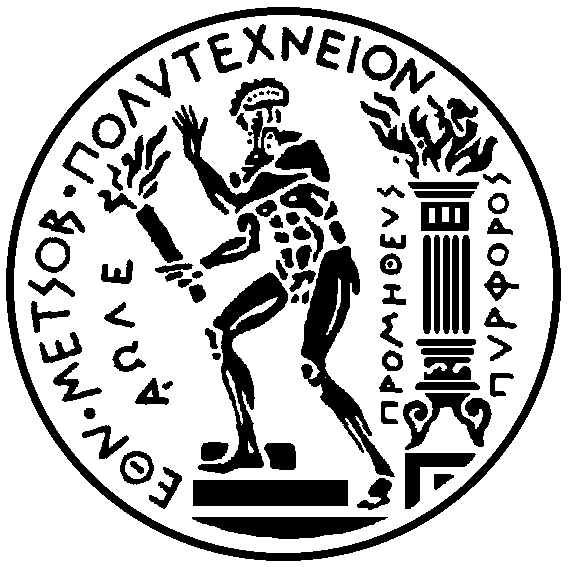
\includegraphics[height=2cm]{pyrforos.png}
        \end{center}
\end{frame}

\section*{Επισκόπηση}

\begin{frame}
  \tableofcontents[hidesubsections]
\end{frame}

\section{Πρωταρχικά αναδρομικές συναρτήσεις}

\subsection{Ορισμός}

\begin{frame}
        \frametitle{Ορισμός}
        \begin{itemize}
                \item   Οι \textbf{πρωταρχικά αναδρομικές συναρτήσεις} 
                                είναι συναρτήσεις με πεδίο ορισμού το \( \mathbb{N}^k \) 
                                και σύνολο τιμών το \( \mathbb{N} \).
                \pause
                \item   Η κλάση τους είναι η μικρότερη που περιέχει τις ακόλουθες
                                θεμελιώδεις συναρτήσεις και είναι κλειστή ως προς τα ακόλουθα
                                σχήματα κλεισίματος.
        \end{itemize}
\end{frame}

\subsection{Θεμελιώδεις συναρτήσεις}

\begin{frame}
        \frametitle{Θεμελιώδεις συναρτήσεις}
        \begin{itemize}
                \item Η σταθερή συνάρτηση με τιμή 0: \[Z_0=0\]
                \pause
                \item Η συνάρτηση που παίρνει έναν αριθμό και επιστρέφει τον επόμενο: \[S_1(n)=n+1\]
                \pause
                \item Οι συναρτήσεις προβολής: \[U^i_n(x_1,\ldots,x_i,\ldots,x_n)=x_i\]
        \end{itemize}
\end{frame}

\subsection{Σχήματα κλεισίματος}

\subsubsection{Σύνθεση}

\begin{frame}
        \frametitle{Σύνθεση}
        \begin{itemize}
                \item Αν έχουμε τις πρωταρχικά αναδρομικές συναρτήσεις: \[H_m, G1_n, \ldots, GM_n\]
                \pause
                \item Τότε και η \[F_n(x_1,\ldots,x_n) = H_m(G1_n(x_1,\ldots,x_n),\ldots,GM_n(x_1,\ldots,x_n))\]
                είναι πρωταρχικά αναδρομική.
        \end{itemize}
\end{frame}

\subsubsection{Πρωταρχική Αναδρομή}

\begin{frame}
        \frametitle{Πρωταρχική Αναδρομή}
        \begin{itemize}
                \item Αν έχουμε τις πρωταρχικά αναδρομικές συναρτήσεις: \[G_n, H_{n+2}\]
                \pause
                \item Τότε και η 
                \[
                        \left\{
                                \begin{array}{ll}
                                        F_n(x_1,\ldots,x_n, 0) &= G_n(x_1,\ldots,x_n) \\
                                        F_n(x_1,\ldots,x_n, S_1(y)) &= H_{n+2}(x_1,\ldots,x_n, y , F_n(x_1,\ldots,x_n, y))
                                \end{array}
                        \right.
                \]
                είναι πρωταρχικά ανδρομική.
        \end{itemize}
\end{frame}

\subsection{Παραδείγματα πρωταρχικά αναδρομικών συναρτήσεων}

\begin{frame}
        \frametitle{Παραδείγματα πρωταρχικά αναδρομικών συναρτήσεων}
        \begin{itemize}
                \item Η συνάρτηση προηγούμενος:
                \[
                        \left\{
                                \begin{array}{ll}
                                        P_1(0) &= Z_0\\
                                        P_1(S_1(x)) &= U^1_2(x,P(x))
                                \end{array}
                        \right.
                \]
                \pause
                \item Η συνάρτηση πρόσθεσης:
                \[
                        \left\{
                                \begin{array}{ll}
                                        Add_2(x, 0) &= U^1_1(x)\\
                                        Add_2(x, S_1(y)) &= S_1(U^3_3(x, y , Add_2(x, y)))
                                \end{array}
                        \right.
                \]
                \pause
                ή πιο απλά:
                \[
                        \left\{
                                \begin{array}{ll}
                                        Add_2(x, 0) &= x\\
                                        Add_2(x, S_1(y)) &= S_1(Add_2(x, y))
                                \end{array}
                        \right.
                \]
                \pause
                \item Η συνάρτηση αφαίρεσης:
                \[
                        \left\{
                                \begin{array}{ll}
                                        Sub_2(x, 0) &= x\\
                                        Sub_2(x, S_1(y)) &= P_1(Sub_2(x, y))
                                \end{array}
                        \right.
                \]
        \end{itemize}
\end{frame}

\begin{frame}
        \frametitle{Παραδείγματα πρωταρχικά αναδρομικών συναρτήσεων}
        \begin{itemize}
                \item Η συνάρτηση πολλαπλασιασμού:
                \[
                        \left\{
                                \begin{array}{ll}
                                        Mult_2(x, 0) &= Z_0\\
                                        Mult_2(x, S_1(y)) &= Add_2(x, Mult_2(x, y))
                                \end{array}
                        \right.
                \]
                \pause
                \item Η συνάρτηση << ίσο με 0 >>:
                \[
                        \left\{
                                \begin{array}{ll}
                                        EZ(0) &= S_1(Z_0)\\
                                        EZ(S_1(x)) &= Z_0
                                \end{array}
                        \right.
                \]
        \end{itemize}
\end{frame}

\subsection{Απαρίθμηση πρωταρχικά αναδρομικών συναρτήσεων}

\begin{frame}
        \frametitle{Απαρίθμηση πρωταρχικά αναδρομικών συναρτήσεων}
        \begin{itemize}
                \item Οι πρωταρχικά αναδρομικές συναρτήσεις είναι αριθμήσιμο σύνολο.
                \pause
                \item Για την απαρίθμηση μπορούμε να χρησιμοποιήσουμε π.χ. το 
                ακόλουθο σχήμα βασισμένο στα αριθμητικά του G\"odel
                \footnote{
                \htmladdnormallink{\tiny
                http://en.wikipedia.org/wiki/G\"odel\_number}
                {http://en.wikipedia.org/wiki/G\%C3\%B6del_number}}:
                \begin{itemize}
                        \item Οι θεμελιώδεις συναρτήσεις:
                        \[
                                \begin{array}{l}
                                        Z_0 \rightarrow 1 \\
                                        S_1 \rightarrow 2*3^1 \\
                                        U^i_n \rightarrow 2^2*3^n*5^i
                                \end{array}
                        \]
                \end{itemize}
        \end{itemize}
\end{frame}

\begin{frame}
        \frametitle{Απαρίθμηση πρωταρχικά αναδρομικών συναρτήσεων}
        \begin{itemize}
                \item Το σχήμα σύνθεσης:
                \begin{itemize}
                        \item Αν έχουμε την αντιστοίχιση:
                                \[\begin{array}{l}
                                        H_m \rightarrow N_H,\\
                                        G1_n \rightarrow N_{G1},\\
                                        \ldots,\\
                                        GM_n \rightarrow N_{GM}
                                \end{array}\]
                \pause
                        \item Τότε η \( F_n(x_1,\ldots,x_n) = H_m(G1_n(x_1,\ldots,x_n),\ldots,GM_n(x_1,\ldots,x_n)) \)
                        αντιστοιχεί στο:
                        \[
                                2^3*3^n*5^{N_H}*7^{N_{G1}}*\ldots*Prime_{m+3}^{N_{GM_n}}
                        \]
                \end{itemize}                   
        \end{itemize}
\end{frame}

\begin{frame}
        \frametitle{Απαρίθμηση πρωταρχικά αναδρομικών συναρτήσεων}
        \begin{itemize}
                \item Το σχήμα πρωταρχικής αναδρομής:
                \begin{itemize}
                        \item Αν έχουμε την αντιστοίχιση:
                                \[\begin{array}{l}
                                        G_n \rightarrow N_Γ,\\
                                        H_{n+2} \rightarrow N_H
                                \end{array}\]
                \pause
                        \item Τότε η 
                        \[\left\{
                                \begin{array}{ll}
                                        F_n(x_1,\ldots,x_n, 0) &= G_n(x_1,\ldots,x_n) \\
                                        F_n(x_1,\ldots,x_n, S_1(y)) &= H_{n+2}(x_1,\ldots,x_n, y , F_n(x_1,\ldots,x_n, y))
                                \end{array}
                        \right.\]
                        αντιστοιχεί στο:
                        \[
                                2^4*3^n*5^{N_G}*7^{H_H}
                        \]
                \end{itemize}                   
        \end{itemize}
\end{frame}

\begin{frame}
        \frametitle{Απαρίθμηση πρωταρχικά αναδρομικών συναρτήσεων}
        \begin{itemize}
                \item Η απαρίθμηση δεν αντιστοιχεί σε κάθε ακέραιο μια έγκυρη
                πρωταρχικά αναδρομική συνάρτηση αλλά είναι εφικτό να ελεγχθεί αν
                ένας ακέραιος αντιστοιχεί σε έγκυρη συνάρτηση:
                \pause
                \begin{itemize}
                        \item Παραγοντοποιούμε τον αριθμό
                \pause
                        \item Ελέγχουμε τη δύναμη του 2 για να δούμε αν είναι απλή περίπτωση
                \pause
                        \item Αν είναι σχήμα κλεισίματος, ελέγχουμε αναδρομικά κάθε μια συνάρτηση
                        που περιλαμβάνεται όπως και το ίδιο το σχήμα κλεισίματος.
                \end{itemize}
                \pause
                \item Είναι επίσης εύκολο να βρούμε πόσα ορίσματα εχει μια συνάρτηση που αντιστοιχεί σε έναν κωδικό
                \pause
                \item \(Legal(x)=0|1\) και \(Args(x)=n\)
        \end{itemize}
\end{frame}

\section{Αναδρομικές συναρτήσεις}

\subsection{Γιατί δεν αρκεί η πρωταρχική αναδρομή}

\begin{frame}
        \frametitle{Γιατί δεν αρκεί η πρωταρχική αναδρομή}
        \begin{itemize}
                \item Δεν είναι όλες οι << υπολογίσιμες >> συναρτήσεις
                πρωταρχικά αναδρομικές!
                \pause
                \item Έστω η συνάρτηση \(f(x)\) με τύπο:
                \[f(x)=\left\{
                        \begin{array}{ll}
                                0 &, Legal(x) \neq 1 \wedge Args(x) = 1\\
                                FX_1(x) + 1 &, otherwise
                        \end{array}
                \right.\]
                όπου \(FX_1\) η συνάρτηση με κωδικό \(x\).
                \pause
                \item Υπολογίσιμη συνάρτηση.
        \end{itemize}
\end{frame}

\begin{frame}
        \frametitle{Γιατί δεν αρκεί η πρωταρχική αναδρομή}
        \begin{itemize}
                \item Έστω ότι η \(f\) είναι πρωταρχικά αναδρομική.
                \pause
                \item Τότε έχει κάποιον κωδικό έστω \(N_f\).
                \pause
                \item Άρα \(f(N_f) = FN_f(N_f) + 1 = f(N_f) + 1\).
                \pause
                \item Άτοπο!
        \end{itemize}
\end{frame}

\begin{frame}
        \frametitle{Γιατί δεν αρκεί η πρωταρχική αναδρομή}
        \begin{itemize}
                \item Η συνάρτηση Ackermann:
                \[\left\{
                        \begin{array}{ll}
                                A(0,n) &= n+1\\
                                A(m,0) &= A(m-1,1)\\
                                A(m,n) &= A(m-1, A(m,n-1))
                        \end{array}
                \right.\]
                \pause
                \item Υπολογίσιμη.
                \pause
                \item Δεν μπορεί να γραφεί με πρωταρχική αναδρομή 
                \footnote{
                \htmladdnormallink{\tiny
                http://home.manhattan.edu/~gregory.taylor/thcomp/pdf-files/ackerman.pdf}
                {http://home.manhattan.edu/~gregory.taylor/thcomp/pdf-files/ackerman.pdf}}.
        \end{itemize}
\end{frame}

\subsection{Αναδρομικές συναρτήσεις}

\begin{frame}
        \frametitle{Αναδρομικές συναρτήσεις}
        \begin{itemize}
                \item Μερικές συναρτήσεις.
                \[F_n(a_1,\ldots,a_n)=\left\{
                        \begin{array}{l}
                                b\\
                                \bot
                        \end{array}
                \right.\]
                \pause 
                \item Περιλαμβάνουν:
                \begin{itemize}
                        \item Θεμελιώδεις συναρτήσεις.
                        \pause
                        \item Σχήματα κλεισίματος:
                        \begin{itemize}
                                \item Σύνθεση
                                \item Πρωταρχική αναδρομή
                                \pause
                                \item \textbf{Ελαχιστοποίηση}
                        \end{itemize}
                \end{itemize}
        \end{itemize}
\end{frame}

\subsection{Σχήμα ελαχιστοποίησης}

\begin{frame}
        \frametitle{Σχήμα ελαχιστοποίησης}
        \begin{itemize}
                \item Αν έχουμε την αναδρομική συνάρτηση \(F_{n+1}(y,x_1,\ldots,x_n)\)
                \pause
                \item Τότε και η:
                \[
                \small
                \begin{array}{ll}
                G_n =\\
                \mu y(x_1,\ldots,x_n) = z \Leftrightarrow 
                & \exists y_0,\ldots,y_n\:such\:that \\
                & y_i = F_{n+1}(i, x_1,\ldots, x_n),\:for\:i=0,1,\ldots,z \\
                & y_i > 0,\:for\:i=0,1,\ldots,z-1 \\
                & y_z = 0
                \end{array}
                \]
                είναι αναδρομική.
        \end{itemize}
\end{frame}

\subsection{Αοριστία}

\begin{frame}
        \frametitle{Αοριστία}
        \begin{itemize}
    	    \item Η χρήση του παραπάνω σχήματος εισάγει αοριστίες:
    	    \pause
            \item Αν \( y_i = F_{n+1}(i, x_1,\ldots, x_n) \) δεν είναι ποτέ ίσο με \( 0 \).
            \pause
            \item Αν \( y_i > 0,\:for\:i=0,1,\ldots,w-1 \) και \( y_w \) δεν ορίζεται.
        \end{itemize}
\end{frame}

\subsection{Παραδείγματα αναδρομικών συναρτήσεων}

\begin{frame}
        \frametitle{Παραδείγματα αναδρομικών συναρτήσεων}
        \begin{itemize}
                \item Αναπαράσταση της συνάρτησης Ackermann με αναδρομή
        \end{itemize}
\end{frame}

\section{Στοιχεία λ-λογισμού}

\subsection{Συντακτικό}

\begin{frame}
        \frametitle{Συντακτικό}
        \begin{itemize}
                \item Ένας λ-όρος μπορεί να είναι μια μεταβλητή.\[x\]
                \pause
                \item Αν \(t\) είναι λ-όρος και \(x\) είναι μεταβλητή, τότε \[\lambda x . t\]
                είναι επίσης λ-όρος.
                \pause
                \item Αν \(t, u\) είναι λ-όροι, τότε \[(t)u\]
                είναι επίσης λ-όρος.
        \end{itemize}
\end{frame}

\subsection{Αντικατάσταση}

\begin{frame}
        \frametitle{Αντικατάσταση}
        \begin{itemize}
        	\item 
        	\item Αν \(t\) είναι λ-όρος και \(x\) είναι μεταβλητή, τότε η αντικατάσταση της \(x\)
            από τον \(t\)
        \end{itemize}
\end{frame}

\begin{frame}
        \frametitle{}
        \begin{itemize}
                \item
        \end{itemize}
\end{frame}

\subsection{β-συστολή}
\subsection{β-αναγωγή}
\subsection{β-ισοδυναμία}
\subsection{Κανονικοποίηση}

\section{Αναπαράσταση αναδρομικών συναρτήσεων}

\subsection{Church Numerals}

\begin{frame}
        \frametitle{Church Numerals}
        \begin{itemize}
                \item Αναπαράσταση του \( \mathbb{N} \) στο λ-λογισμό:
                \pause
	        	\[ \begin{array}{l}
	        		0 \rightarrow \lambda f . \lambda x . x \\
	        		1 \rightarrow \lambda f . \lambda x . (f) x \\
	        		2 \rightarrow \lambda f . \lambda x . (f) (f) x \\
	        		\ldots \\
	        		n \rightarrow \lambda f . \lambda x . \underbrace{(f) \ldots (f)}_n x \\
	        		\ldots
	        	\end{array} \]
	        	\pause
                \item Αν \(n \) είναι Church Numeral και \(t, u\) είναι λ-όροι, τότε
                \[ n\:t\:u =_\beta (t)^n u \]
        \end{itemize}
\end{frame}

\subsection{Θεμελιώδεις συναρτήσεις}
\subsection{Σχήματα κλεισίματος}
\subsubsection{Σύνθεση}
\subsubsection{Πρωταρχική Αναδρομή}
\subsection{Σχήμα ελαχιστοποίησης}
\end{document}
